% appendices/lyttle21.tex
%
% Copyright 2023 Alexander Lyttle.
%
% This work may be distributed and/or modified under the conditions of the
% LaTeX Project Public License (LPPL) version 1.3 or later.
%
% The latest version of this license is in
% https://www.latex-project.org/lppl.txt and version 1.3 or later is part of
% all distributions of LaTeX version 2005/12/01 or later.
%
%
\chapter[Hierarchically Modelling Dwarf and Subgiant Stars]{Hierarchically Modelling \emph{Kepler} Dwarfs and Subgiants to Improve Inference of Stellar Properties with Asteroseismology}\label{apx:hmd}

\textit{%
    In this chapter, I present the appendix of \citet{Lyttle.Davies.ea2021} with minor modification. It follows from, and is referenced to, in Chapter \ref{chap:hmd}. Firstly, I explain the methodology behind the neural network emulator in Section \ref{sec:ann}. In Section \ref{sec:beta}, I briefly show the beta distribution which was used as a prior for some parameters in the main body of work. Finally, I test the hierarchical model on a synthetic population of stars in Section \ref{sec:test-stars}.
}

\section{Artificial Neural Network}\label{sec:ann}

%%%%%%%%%%%%%%%%%%%%%%%%%%%%%%%%%%%%%%%%%%%%%%%%%%

%%%%%%%%%%% ARTIFICIAL NEURAL NETWORK %%%%%%%%%%%%

Once we constructed our grid of models, we needed a way to continuously sample the grid for use in our statistical model. We opted to train an Artificial Neural Network (ANN). The ANN is advantageous over interpolation because it scales well with dimensionality, training and evaluation is fast, and gradient evaluation is easy due to its roots in linear algebra \citep{Haykin2007}. We trained an ANN on the data generated by the grid of stellar models to map fundamentals to observables. Firstly, we split the grid into a \emph{train} and \emph{validation} dataset for tuning the ANN, as described in Appendix \ref{sec:train}. We then tested a multitude of ANN configurations and training data inputs, repeatedly evaluating them with the validation dataset in Appendix \ref{sec:opt}. In Appendix \ref{sec:test}, we reserved a set of randomly generated, off-grid stellar models as our final \emph{test} dataset to evaluate the approximation ability of the best-performing ANN independently from our train and validation data. Here, we briefly describe the theory and motivation behind the ANN.

An ANN is a network of artificial \emph{neurons} which each transform an input vector, $\boldsymbol{x}$ based on trainable weights, $\boldsymbol{w}$ and a bias, $b$. The weights are represented by the connections between neurons and the bias is a unique scalar associated with each neuron. A multi-layered ANN is where neurons are arranged into a series of layers such that any neuron in layer $j-1$ is connected to at least one of the neurons in layer $j$. 

\begin{figure}
    \centering
    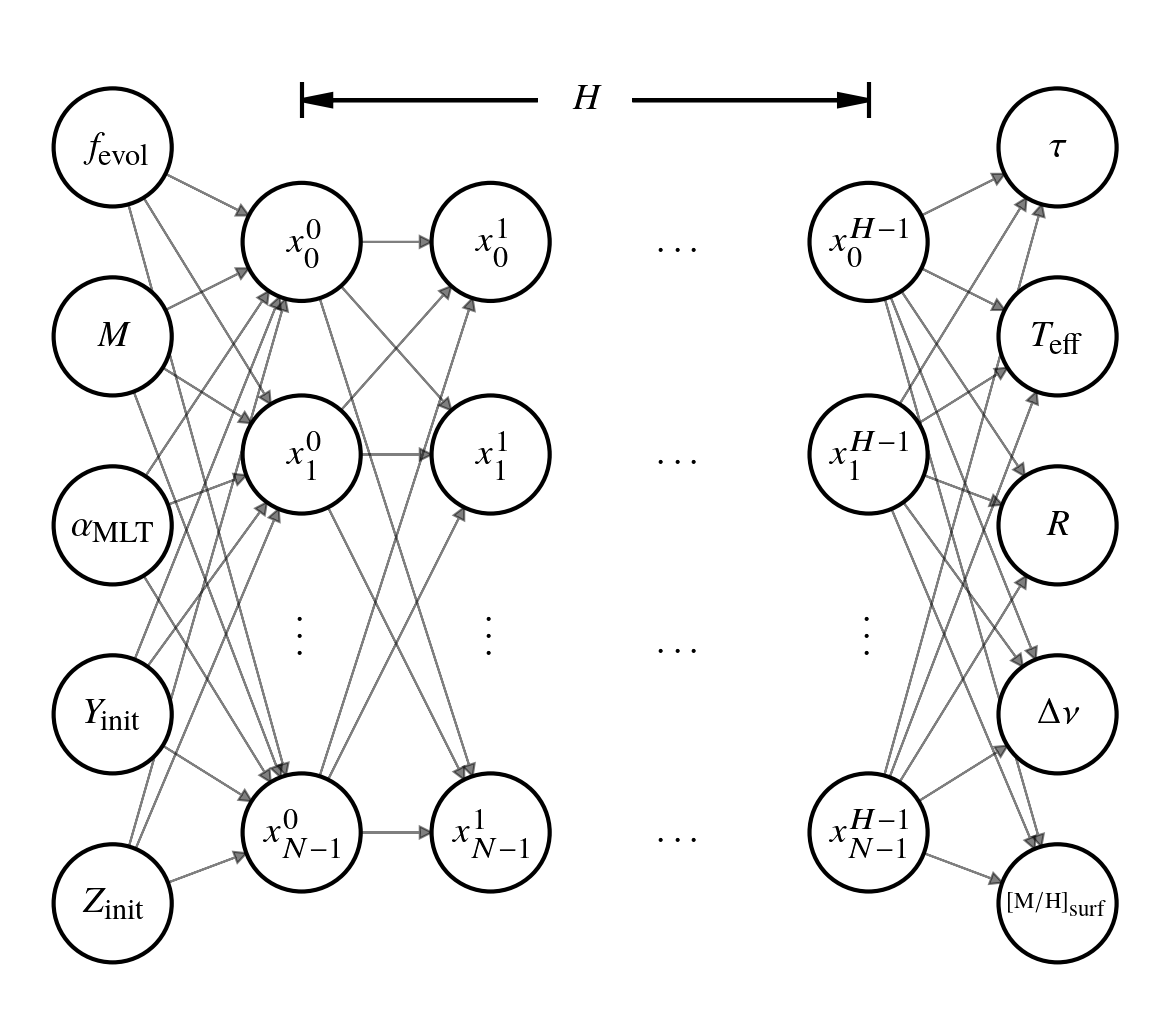
\includegraphics{figures/network_10.png}
    \caption[An artificial neural network comprising $H$ hidden layers with $N$ neurons per layer.]{An artificial neural network comprising $H$ hidden layers with $N$ neurons per layer. Arrows connecting the nodes represent tunable weights.}
    \label{fig:net}
\end{figure}

In this work, we considered a fully-connected ANN, where each neuron in layer $j-1$ is connected to every neuron in layer $j$. The output of the $k$-th neuron in layer $j$ is, 
%
\begin{equation}
    x_{j, k}=f_j(\boldsymbol{w}_{j, k} \cdot \boldsymbol{x}_{j-1} + b_{j, k}),
\end{equation}
%
where $f_j$ is the \emph{activation} function for the $j$-th layer, $\boldsymbol{w}_{j, k}$ are the weights connecting all the neurons in layer $j-1$ to the current neuron, and $b_{j, k}$ is the bias. This generalises such that the output of the $j$-th layer is,
%
\begin{equation}
    \boldsymbol{x}_{j}=f_j(\boldsymbol{W}_{j} \cdot \boldsymbol{x}_{j-1} + \boldsymbol{b}_{j}),
\end{equation}
%
where $\boldsymbol{W}_j$ is the matrix of weights leading to all neurons in the $j$-th layer. For a regression ANN, we typically have a linear activation function applied to the final output layer. Layers of neurons between the input and output layers are called \emph{hidden} layers. Therefore, the output of a network of $H$ hidden layers with initial input $\boldsymbol{\mathbb{X}}$ is,
%
\begin{equation}
    \widetilde{\boldsymbol{\mathbb{Y}}} = \boldsymbol{W}_{H} \cdot f_{H-1}(\dots f_1(\boldsymbol{W}_1 \cdot f_0(\boldsymbol{W}_{0} \cdot \boldsymbol{\mathbb{X}} + \boldsymbol{b}_{0}) + \boldsymbol{b}_1) ) + \boldsymbol{b}_{H}.
\end{equation}
%
We also restricted our configuration to an ANN with the same number of neurons, $N$ in each hidden layer. Hereafter, we refer to our choice of neurons per layer, $N$ and hidden layers, $H$ as the \emph{architecture} (see Fig. \ref{fig:net}).

To fit the ANN, we used a set of training data, $\boldsymbol{\mathbb{D}}_\mathrm{train} = \{\boldsymbol{\mathbb{X}}_i, \boldsymbol{\mathbb{Y}}_i\}_{i=1}^{N_\mathrm{train}}$ comprising $N_\mathrm{train}$ input-output pairs. We split the training data into pseudo-random batches, $\boldsymbol{\mathbb{D}}_\mathrm{batch}$ because this has been shown to improve ANN stability and computational efficiency \citep{Masters.Luschi2018}. The set of predictions made for each batch is evaluated using a \emph{loss} function which primarily comprises an error function, $E(\boldsymbol{\mathbb{D}}_\mathrm{batch})$ to quantify the difference between the training data outputs ($\boldsymbol{\mathbb{Y}}$) and predictions ($\widetilde{\boldsymbol{\mathbb{Y}}}$). We also considered an additional term to the loss called \emph{regularisation} which helps reduce over-fitting \citep{Goodfellow.Bengio.ea2016}. During fitting, the weights are updated after each batch using an algorithm called the \emph{optimizer}, back-propagating the error with the goal of minimising the loss such that $\widetilde{\boldsymbol{\mathbb{Y}}} \approx \boldsymbol{\mathbb{Y}}$ \citep[see e.g.][]{Rumelhart.Hinton.ea1986}.

We trained the ANN using \textsc{TensorFlow} \citep{Abadi.Barham.ea2016}. We varied the architecture, number of batches, choice of loss function, optimizer, and regularisation during the optimisation phase. For each set of ANN parameters, we initialised the ANN with a random set of weights and biases and minimised the loss over a given number of \emph{epochs}. An epoch is defined as one iteration through the entire training dataset, $\boldsymbol{\mathbb{D}}_\mathrm{train}$. We tracked the loss for each ANN using an independent validation dataset to determine the most effective choice of ANN parameters (see Appendix \ref{sec:opt}).

\subsection{Train, Validation, and Test Data}\label{sec:train}

%%%%%%%%%%%%%%%%%%%%%%%%%%%%%%%%%%%%%%%%%%%%%%%%%%

%%%%%%%%%%%%%%%% TRAIN-TEST SPLIT %%%%%%%%%%%%%%%%

We built the train and validation datasets from the outputs of the grid of stellar models in Section \ref{sec:grid}. This included the input parameters: $M$, $\mlt$, $Y_\mathrm{init}$, and the initial heavy-elements fraction, $Z_\mathrm{init}$. We also included the $\teff$, $\log g$, $\dnu$, stellar age ($\tau$), radius ($R$), surface metallicity ($\metallicity_\mathrm{surf}$), and other chemical composition information generated by the models. We determined the fractional MS lifetime, $f_{\mathrm{MS}} = \tau / \tau_{\mathrm{MS}}$, of each evolutionary track by taking $\tau_{\mathrm{MS}}$ as the age when the central hydrogen fraction, $X_c < 0.01$. We then cut data where $f_{\mathrm{MS}} < 0.01$ to remove points on the grid prior to the MS. Once we had refined the data from the grid of models, we randomly sampled \num{7.736e6} points to use as the training dataset, with the remaining $\sim \num{2e6}$ points given to the validation dataset. We varied our choice of ANN input and output parameters among those available in the dataset during tuning (see Appendix \ref{sec:opt}).

Additionally, we produced a test dataset of $\sim \num{2e6}$ stellar models evolved using \textsc{MESA}. Values for the initial $M$, $\metallicity$, $Y$, and $\mlt$ were chosen randomly within the range of grid parameters described in Table \ref{tab:grid} such that they spanned the breadth of the grid in an unbiased manner. We prepared this dataset in the same way as the training set, but also constrained it to $\tau < \SI{15}{\giga\year}$ because we consider ages above $\sim \SI{15}{\giga\year}$ unphysical and such points are sparse in the training data. The test dataset was set aside and evaluated on the final ANN.

\subsection{Tuning}\label{sec:opt}

%%%%%%%%%%%%%%%%%%%%%%%%%%%%%%%%%%%%%%%%%%%%%%%%%%

%%%%%%%%%%%%%%%%%% OPTIMIZATION %%%%%%%%%%%%%%%%%%

We trained an ANN to reproduce stellar observables according to our choice of physics with greater accuracy than typical observational precisions. We experimented with a variety of ANN parameter choices, such as the architecture, activation function, optimisation algorithm, and loss function. We tuned the ANN parameters by varying them in both a grid-based and heuristic approach, each time evaluating the accuracy using the validation dataset.

During initial tuning, we found that having stellar age as an input was unstable, because it varied heavily with the other input parameters. We mitigated this by introducing an input to describe the fraction of time a star had spent in a given evolutionary phase, $f_\mathrm{evol}$. 
%
\begin{equation}
    f_\mathrm{evol} = \begin{cases}
        f_\mathrm{MS},\quad &f_\mathrm{MS} \leq 1\\
        1 + \frac{\tau\,-\,\tau_\mathrm{MS}}{\tau_\mathrm{end}\,-\,\tau_\mathrm{MS}},\quad &f_\mathrm{MS} > 1
    \end{cases}\label{eq:fevol}
\end{equation}
%
where $\tau_\mathrm{end}$ is the age of the star at the end of the track,
%
\begin{equation}
    f_\mathrm{MS} = \frac{\tau}{\tau_\mathrm{MS}},
\end{equation}
%
and $\tau_\mathrm{MS}$ is the MS lifetime. A star with $0.01 < f_\mathrm{evol} \leq 1.0$ is in its MS phase, burning hydrogen in its core, and $1.0 < f_\mathrm{evol} \leq 2.0$ has left the MS. Consequently, $f_\mathrm{evol}$ gives the ANN information about the internal state of the star which affects the output observables. Otherwise, $f_\mathrm{evol}$ has little physical meaning, although it could be interpreted as a measure of the evolutionary phase of the star.

We also observed that the ANN trained poorly in areas with a high rate of change in observables, likely because of poor grid coverage in those areas. To bias training to such areas, we calculated the gradient in $\teff$ and $\log g$ between each point for each stellar evolutionary track and used them as optional weights to the loss during tuning. These weights multiplied the difference between the ANN prediction and the training data in our chosen loss function.

After preliminary tuning, we chose the ANN input and output parameters to be $\boldsymbol{\mathbb{X}} = \{f_\mathrm{evol}, M, \mlt, Y_\mathrm{init}, Z_\mathrm{init}\}$ and $\boldsymbol{\mathbb{Y}} = \{\log(\tau), \teff, R, \dnu, \metallicity_\mathrm{surf}\}$ respectively. A generalised form of our neural network is depicted in Fig. \ref{fig:net}. The inputs corresponded to initial conditions in the stellar modelling code and the outputs corresponded to surface conditions throughout the lifetime of the star, except for age which is mapped from $f_\mathrm{evol}$.

We standardised the training dataset by subtracting the median, $\mu_{1/2}$ and dividing by the standard deviation, $\sigma$ for each input and output parameter. We found that the ANN performed better when the training data was scaled in this way as opposed to no scaling at all. We present the parameters used to standardise the training dataset in Table \ref{tab:std}.

\begin{table}
    \centering
    \caption[The median and standard deviation for each parameter in the training data, used to standardise the dataset.]{The median, $\mu_{1/2}$ and standard deviation, $\sigma$ for each parameter in the training data, used to standardise the dataset.}
    \label{tab:std}
    \begin{tabular}{lcccccccccc}
\toprule
{} & \multicolumn{5}{c}{Input} & \multicolumn{5}{c}{Output} \\
{} & $f_\mathrm{evol}$ & $M\,(\si{\solarmass})$ & $\mlt$ & $Y_\mathrm{init}$ & $Z_\mathrm{init}$ & $\log(\tau/\si{\giga\year})$ & $\teff\,(\si{\kelvin})$ & $R\,(\si{\solarradius})$ & $\dnu\,(\si{\micro\hertz})$ & $\metallicity_\mathrm{surf}\,(\si{\dex})$ \\
\midrule
$\mu_{1/2}$ &             0.865 &                  1.000 &  1.900 &             0.280 &             0.017 &                        0.790 &                5566.772 &                    1.224 &                     100.720 &                                     0.081 \\
$\sigma$    &             0.651 &                  0.118 &  0.338 &             0.028 &             0.011 &                        0.467 &                 601.172 &                    0.503 &                      42.582 &                                     0.361 \\
\bottomrule
\end{tabular}

\end{table}

We found that the optimal choice of architecture ($N$ and $H$) varied depending on our choice of other ANN parameters. Therefore, each time we explored a new parameter, we trained an ANN with a grid of $(N,H)$ ranging from $(32, 2)$ to $(512, 10)$.

We evaluated the performance of three activation functions: the hyperbolic-tangent, the rectified linear unit \citep[ReLU;][]{Hahnloser.Sarpeshkar.ea2000, Glorot.Bordes.ea2011} and the exponential linear unit \citep[ELU;][]{Clevert.Unterthiner.ea2015}. Although the ReLU activation function out-performed the other two in speed and accuracy, the resulting ANN output was not smooth. The discontinuity in the ReLU function, $f(x) = \max(0, x)$ in turn caused the output to be discontinuous. This made the ANN difficult to sample for our choice of statistical model (see Section \ref{sec:hbm}). Out of the remaining activation functions, ELU performed the best, providing a smooth output which was well-suited to our probabilistic sampling methods.

We compared the performance of two optimisers: Adam \citep{Kingma.Ba2014} and stochastic gradient descent \citep[SGD; see e.g.][]{Ruder2016} with and without momentum \citep{Qian1999}. Both optimizers required a choice of \emph{learning rate} which determined the rate at which the weights were adjusted during training. We found that Adam performed well, but the validation loss was noisy as a function of epochs as it struggled to converge. The SGD optimizer was less noisy than Adam, but it was difficult to tune the learning rate. However, SGD with momentum allowed for more adaptive weight updates and out-performed the other configurations.

There are several ways to reduce over-fitting, from minimising the complexity of the architecture, to increasing the size and coverage of the training dataset. One alternative is to introduce weight regularisation. So-called L2 regularisation adds a term, $\sim \lambda_k \sum_i w_{i, k}^2$ to the loss function for a given hidden layer, $k$ which acts to keep the weights small. We varied the magnitude of $\lambda_k$ and found that if it was too large it would dominate the loss function, but if it was too small then performance on the validation dataset was poorer.

We compared the choice of two error functions: mean squared error (MSE) and mean absolute error (MAE). The former is widely used among ANNs because it is more sensitive to large errors. However, we tracked both metrics regardless of which was added to the loss function and found that MAE converged faster. Although MAE is less effective at large errors, we found that these were typically at the edges of the grid and the accuracy was good enough everywhere else.

\begin{figure}[tb]
    \centering
    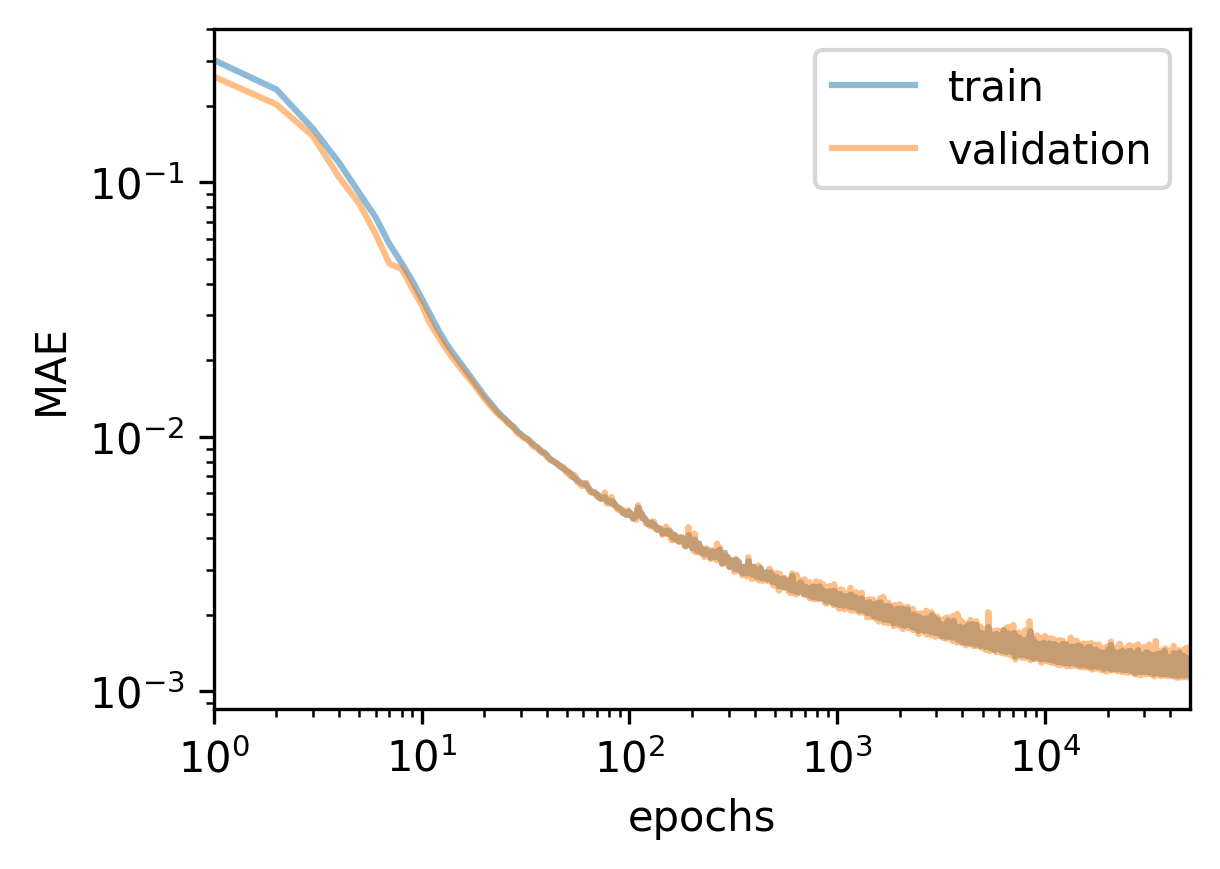
\includegraphics{figures/loss.png}
    \caption{The MAE as a function of epochs for the train and validation datasets.}
    \label{fig:loss}
\end{figure}

After extensive tuning, we opted for an ANN with $N=128$ neurons in each of $H=6$ hidden layers. Each of the hidden layers used an ELU activation function and L2 weight regularisation with $\lambda = \num{1e-6}$. We trained the ANN for \num{50000} epochs with a \num{500} training data batches each containing \num{15472} input-output pairs. To fit the ANN, we used an SGD optimiser with an initial learning rate of \num{1e-4} and momentum of \num{0.999} with an MAE loss function. Training took $\sim \SI{48}{\hour}$ on an NVidia Tesla V100 graphics processing unit (GPU). In Fig. \ref{fig:loss} we show the training and validation MAE as a function of epochs for the final ANN configuration. The training and validation loss were comparable throughout training.

\subsection{Testing}\label{sec:test}

%%%%%%%%%%%%%%%%%%%%%%%%%%%%%%%%%%%%%%%%%%%%%%%%%%

%%%%%%%%%%%%%%%%%%% Validation %%%%%%%%%%%%%%%%%%%

The test dataset contained $\sim \num{2e6}$ stellar models evolved in the same way as the training dataset, but with initial conditions chosen randomly across the range of the grid. We made predictions for the test dataset, deriving luminosity from the output radius and effective temperature, using the final trained ANN as described in Appendix \ref{sec:opt}. We then evaluated the accuracy of the ANN by taking the difference between the test truth and ANN prediction, $x_\mathrm{true} - x_\mathrm{pred}$. 

\begin{figure}[tb]
    \centering
    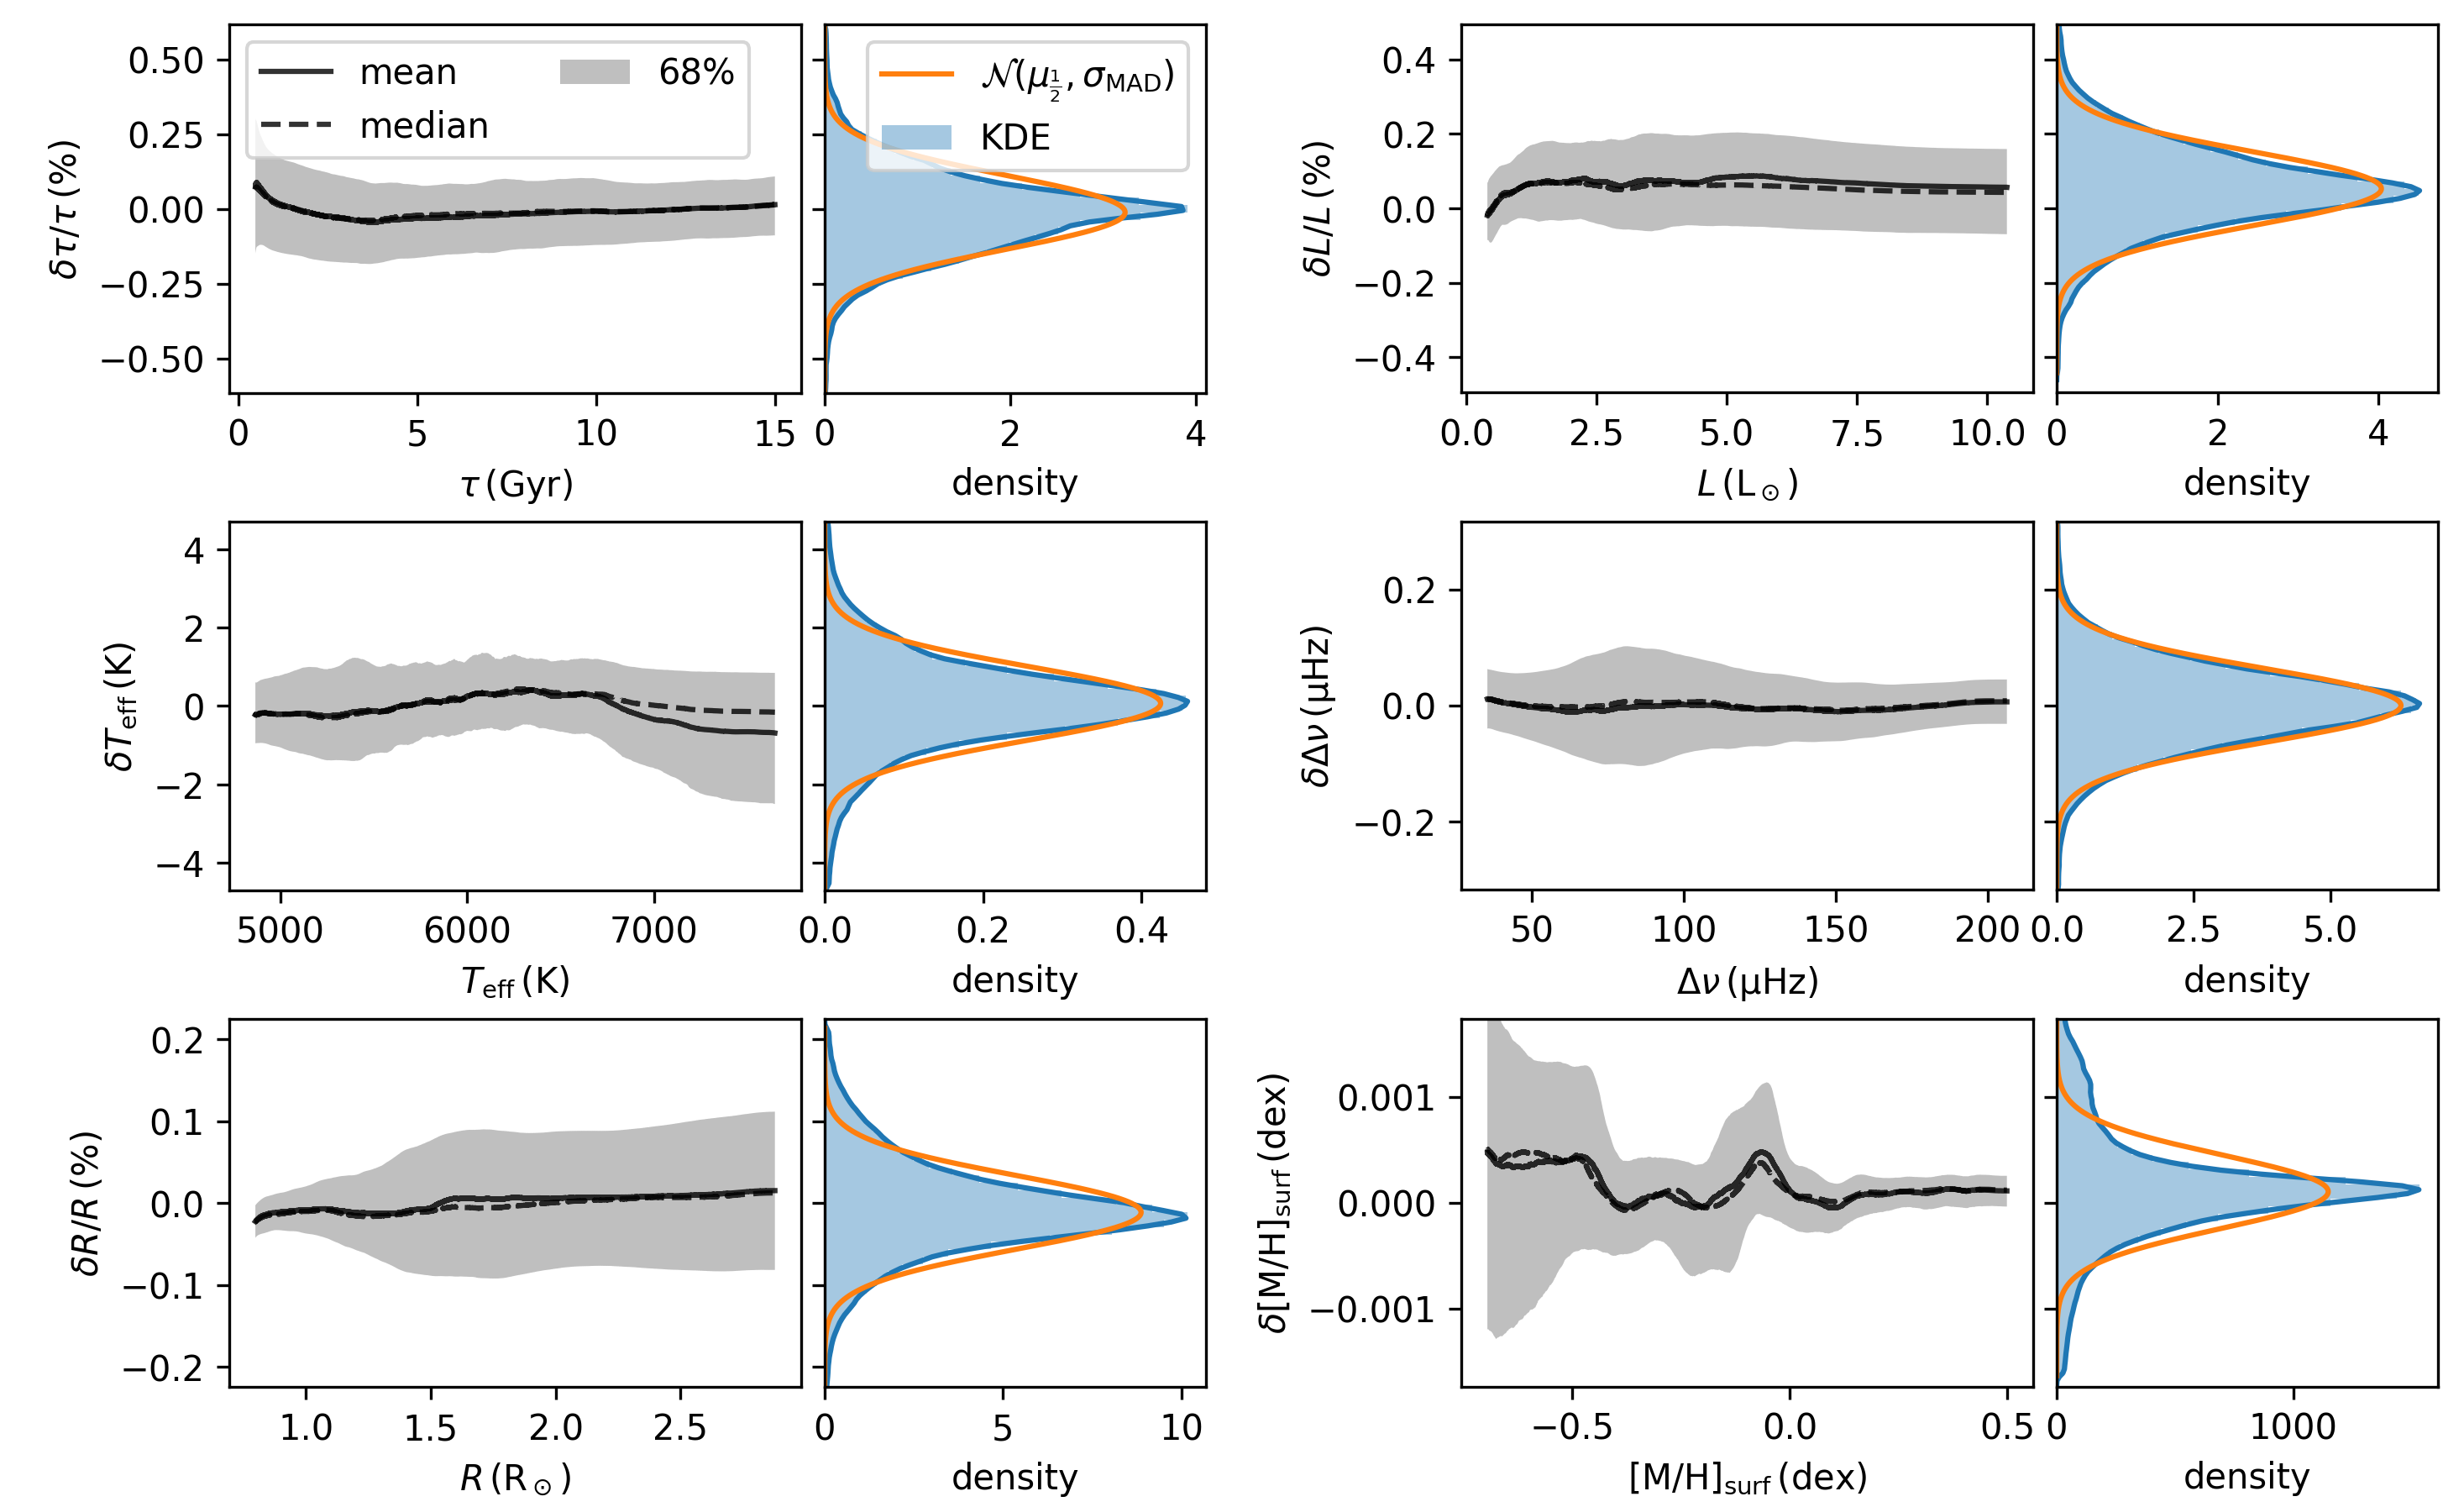
\includegraphics[width=\linewidth]{figures/test_random_wide.png}
    \caption[The error between a given parameter in the test dataset and the ANN prediction for that parameter.]{\emph{Left}: the rolling error between a given parameter in the test dataset ($\mathbb{Y}$) and the ANN prediction for that parameter ($\widetilde{\mathbb{Y}}$) where $\delta \mathbb{Y} = \widetilde{\mathbb{Y}} - \mathbb{Y}$. \emph{Right}: a kernel density estimate (KDE) of the error and a normal distribution centred on the median, $\mu_{1/2}$ with an estimator for the standard deviation from the median absolute deviation, $\sigma_\mathrm{MAD}$.}
    \label{fig:test}
\end{figure}

We found good agreement between the test dataset and ANN predictions, within typical observational uncertainties. We noted that the largest errors lay at the boundaries of the training data and in areas sparsely populated by the grid. This is apparent in Fig. \ref{fig:test} where we plot the test error against each parameter. For example, the spread in error increases for $\metallicity_\mathrm{surf} < -0.5$ where training data is sparse at the edge of the grid. However, the accuracy is very good within the observed range covered by our sample of 81 dwarfs and subgiants. Hence, we chose the median absolute deviation (MAD) as an estimator of the spread in error because it is less sensitive to large errors at the grid boundary than the standard deviation.

\begin{table}
	\centering
	\caption[The median error and median absolute deviation of the error for each ANN output parameter from the test dataset.]{The median error, $\mu_{1/2}$ and median absolute deviation of the error, $\sigma_\mathrm{MAD} = 1.4826\cdot\mathrm{median}(|E(\mathbb{Y}) - \mu_{1/2}|)$ for a given ANN output parameter, $\mathbb{Y}$ from the test dataset. The error, $E(\mathbb{Y})$, is given in the table header, where $\delta \mathbb{Y} = \widetilde{\mathbb{Y}} - \mathbb{Y}$.}
	\label{tab:test}
    \begin{tabular}{lcccccc}
\toprule
Error &  $\delta \tau/\tau\,(\%)$ &  $\delta T_\mathrm{eff}\,(\mathrm{K})$ &  $\delta R/R\,(\%)$ &  $\delta L/L\,(\%)$ &  $\delta \Delta\nu\,(\mathrm{\mu Hz})$ &  $\delta [\mathrm{M}/\mathrm{H}]_\mathrm{surf}\,(\mathrm{dex})$ \\
\midrule
$\mu_{1/2}$           &                    -0.012 &                                  0.070 &              -0.011 &               0.053 &                                0.00022 &                                                         0.00010 \\
$\sigma_\mathrm{MAD}$ &                     0.123 &                                  0.941 &               0.045 &               0.099 &                                0.06341 &                                                         0.00035 \\
\bottomrule
\end{tabular}
    
\end{table}

To represent the accuracy of the ANN, we present the median, $\mu_{1/2}$ and MAD estimator, $\sigma_\mathrm{MAD} = 1.4826\cdot\mathrm{median}(|E(x) - \mu_{1/2}|)$ of the error ($E(x)$) in Table \ref{tab:test}. The median is close to zero for all parameters, showing little systematic bias in the ANN. The MAD is also lower than observational uncertainties quoted in Section \ref{sec:data}. The spread in error for $\dnu$ of $\SI{0.06}{\mu\Hz}$ is comparable to that of observations with the best signal-to-noise. However, the error in $\dnu$ predictions is also comparable to other systematic uncertainties in $\dnu$ discussed in Section \ref{subsec:seismo_model}. Therefore, a robust model which takes account of systematic uncertainties pertaining to $\dnu$, including those from the ANN, will be explored in future work (Carboneau et al. in preparation).

\section{Prior Distributions}\label{sec:beta}

\begin{figure}[tb]
    \centering
    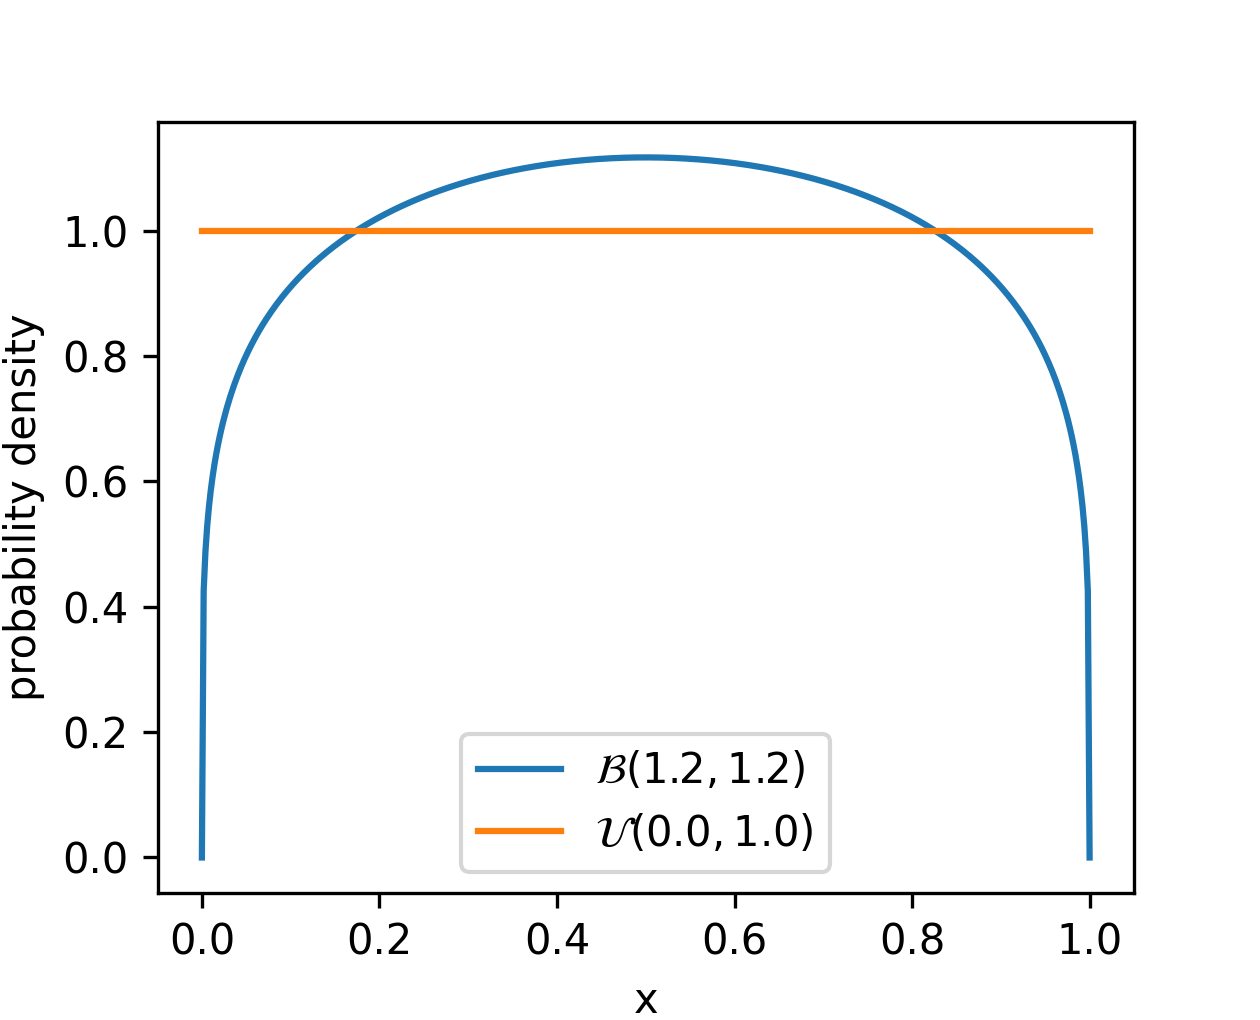
\includegraphics{figures/beta_distribution.png}
    \caption[A beta distribution compared to a uniform distribution.]{A beta distribution ($\mathcal{B}$) with $\alpha = \beta = 1.2$ for some parameter $x$ and a uniform distribution ($\mathcal{U}$) from 0 to 1.}
    \label{fig:beta}
\end{figure}

We chose a transformed beta distribution (see Equation \ref{eq:beta}) as the prior for the non-pooled stellar parameters as an alternative to a uniform distribution. Fig. \ref{fig:beta} shows the beta distribution compared with a uniform distribution for some parameter $x$ from 0 to 1. We found that the continuously differentiable nature of the beta distribution was preferred by the NUTS over the uniform distribution.

\section{The Synthetic Population}\label{sec:test-stars}

%%%%%%%%%%%%%%%%%%%%%%%%%%%%%%%%%%%%%%%%%%%%%%%%%%

%%%%%%%%%%%% THE SYNTHETIC POPULATION %%%%%%%%%%%%

In this section, we present the results for the NP, PP, and MP models run on a synthetic sample of 100 stars with the following initial conditions. We randomly generated initial $M$ and $\metallicity_\mathrm{init}$ uniformly. We drew initial values for $Y_\mathrm{init}$ from a normal distribution centred on the helium enrichment law from Equation \ref{eq:helium} with $\Delta Y / \Delta Z = 1.8$ and $Y_P = 0.247$, and scaled by $\sigma_Y = 0.008$. We also generated initial values for $\mlt$ from a normal distribution centred on $\mu_\alpha = 2.0$ and scaled by $\sigma_\alpha = 0.08$.

We evolved the synthetic stars to randomly chosen ages using \textsc{MESA}. We then took the output $\tau$, $\teff$, $L$, $\dnu$, and $\metallicity_\mathrm{surf}$ from the models and used these as true values for each of the stars. We added random noise to the observed quantities centred on the true values with a standard deviation of 2.2 per cent in $\teff$, 3.5 per cent in $L$, \SI{0.9}{\micro\hertz} in $\dnu$, and \SI{0.07}{\dex} in $\metallicity_\mathrm{surf}$ chosen to be representative of the APOKASC sample.

\subsection{Stellar Parameters}

We found that the NP model recovered the true values for the individual stellar parameters, but the uncertainties were unreliable. The observational quantities alone were not good enough to constrain $Y_\mathrm{init}$ and $\mlt$. As a result, their distributions were truncated at the bounds of their priors. These boundary effects skewed the marginalised posterior means for $Y_\mathrm{init}$ and $\mlt$ towards the centre of the prior (0.28 and 2.0 respectively).

The PP model recovered true values for the synthetic stars with more reliable uncertainty than the NP model. The addition of pooling $Y_\mathrm{init}$ and $\mlt$ between the stars improved their uncertainty which reduced the effects of the prior as seen in the NP model. We found little difference between the results of the PP and MP models.

\begin{figure}[tb]
    \centering
    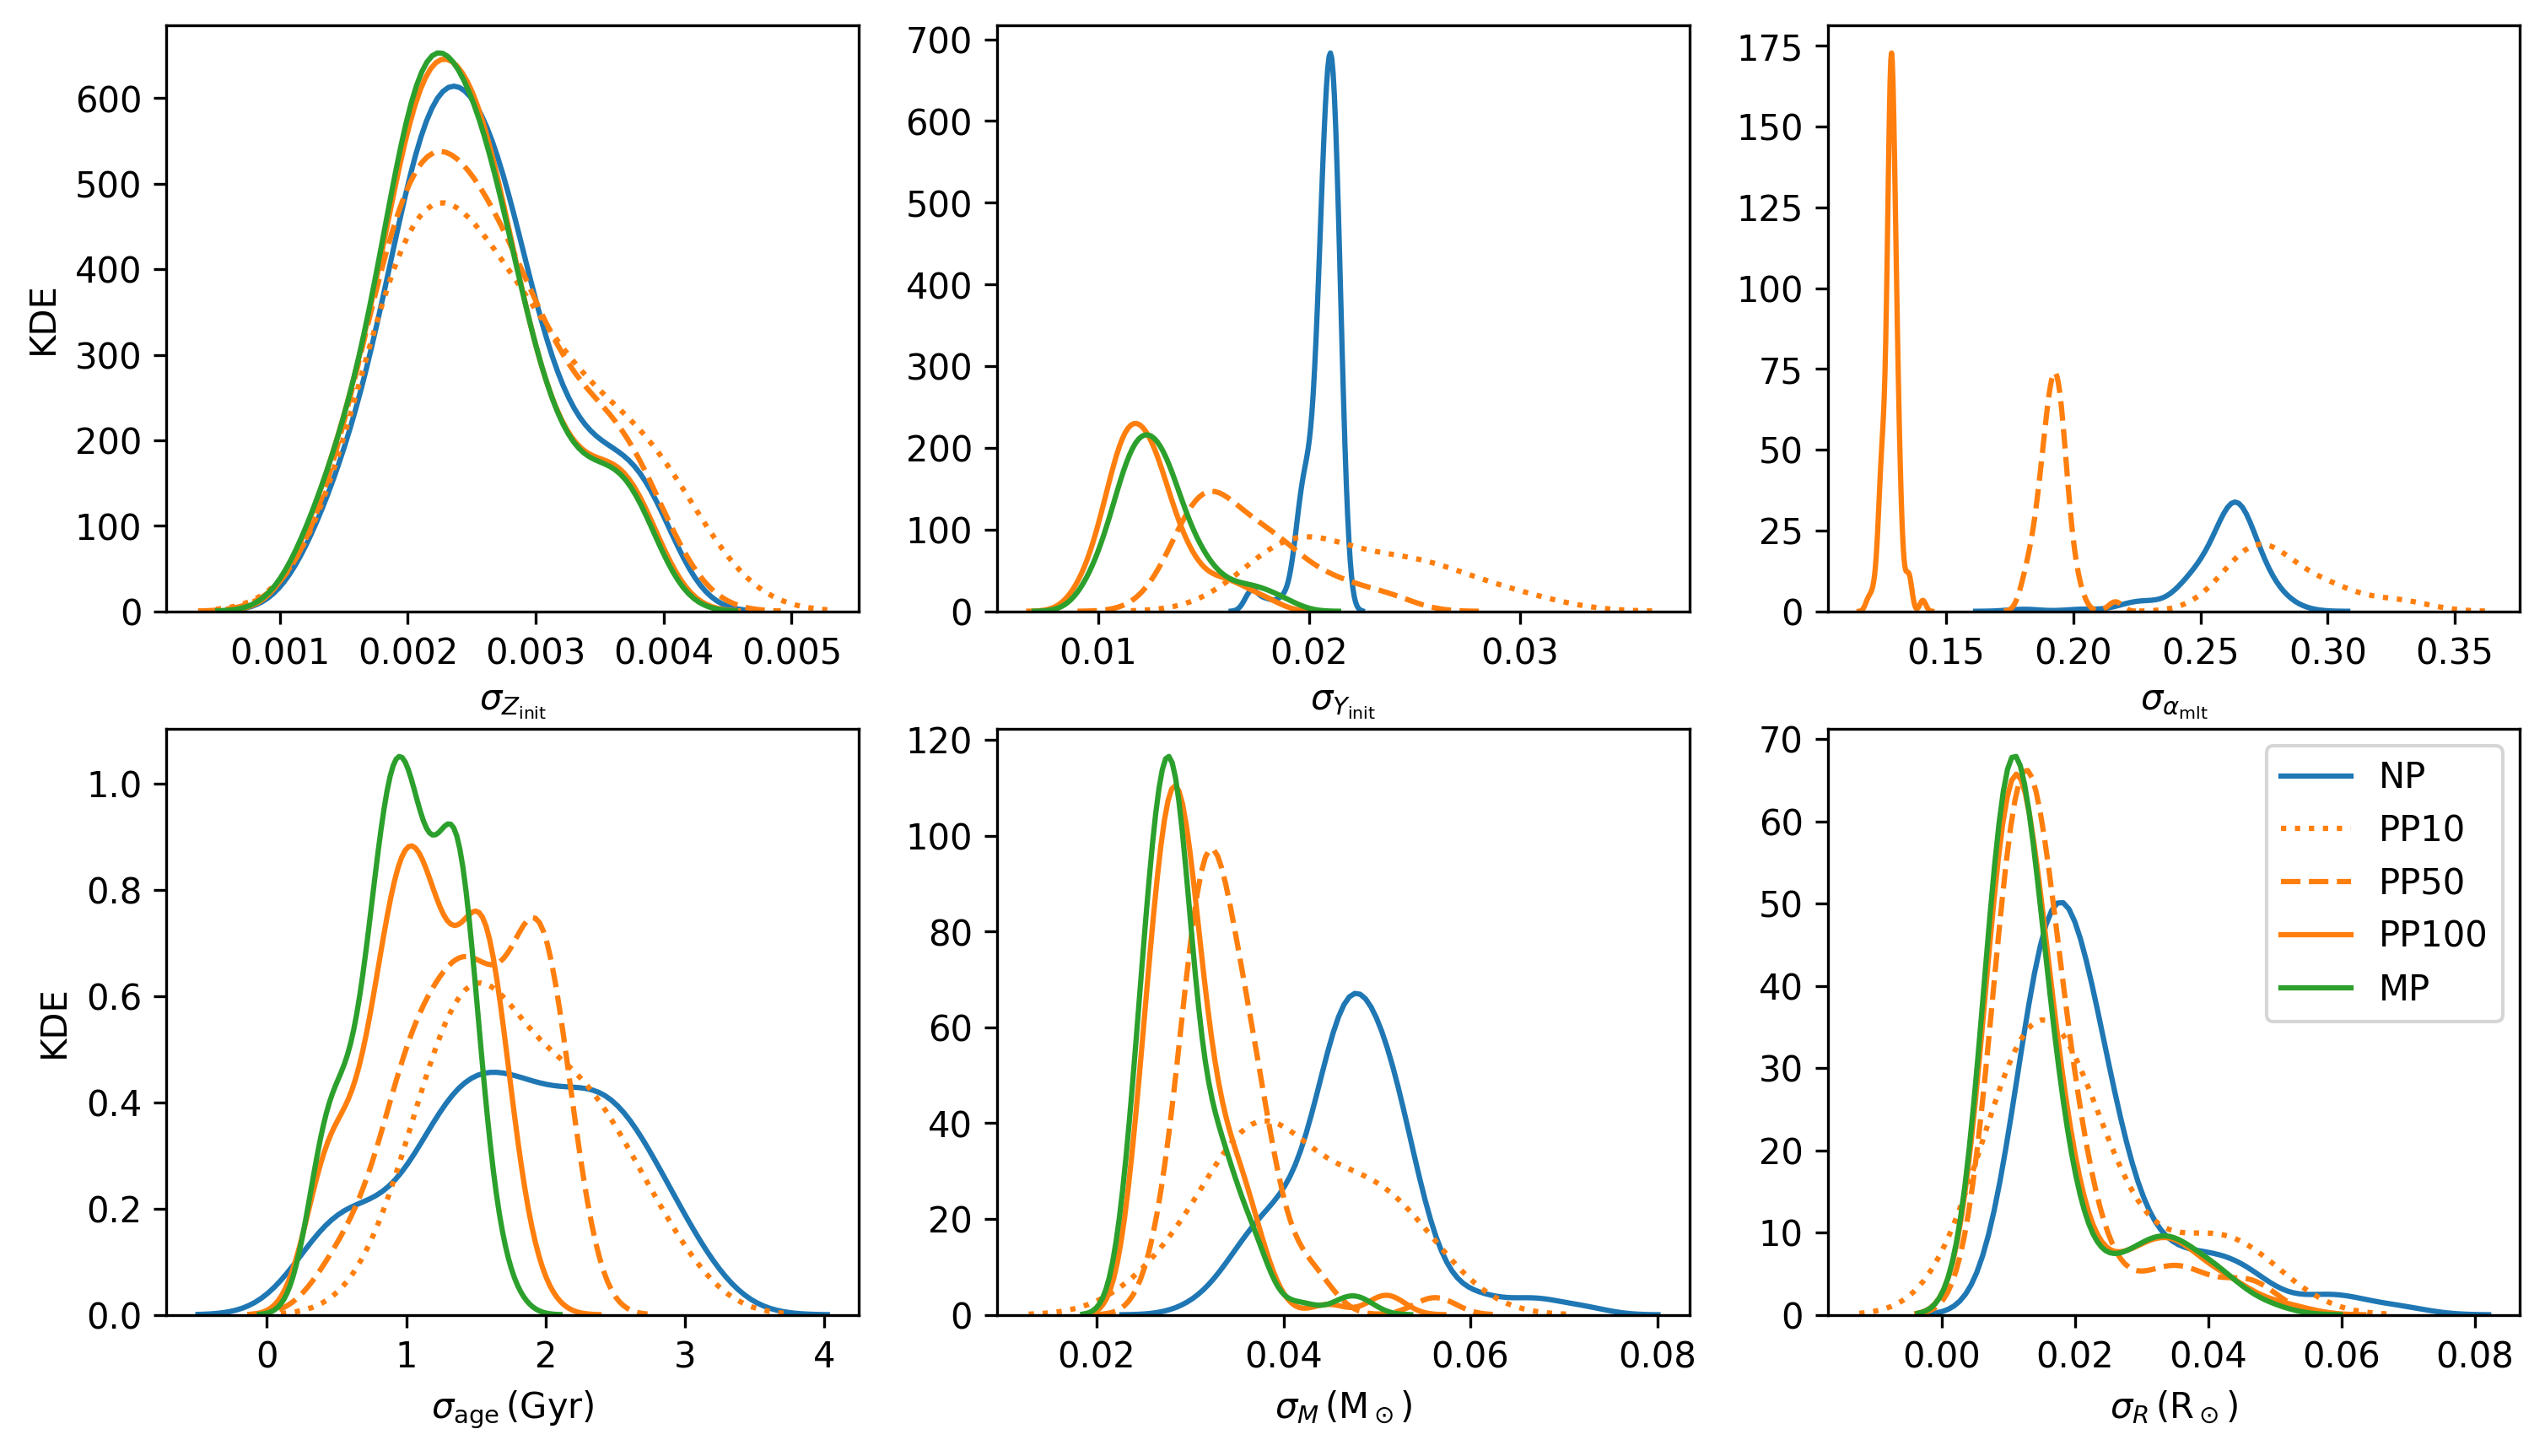
\includegraphics[width=\textwidth]{figures/shrinkage.png}
    \caption[Kernel density estimates of the distributions of statistical uncertainties from each model for the sample of synthetic stars.]{Kernel density estimates (KDEs) of the distributions of statistical uncertainties from each model for the sample of synthetic stars. The PP model was run with 10, 50 and 100 stars and is denoted PP10, PP50, and PP100 respectively. The NP and MP models were both run with the full set of 100 stars.}
    \label{fig:shrinkage}
\end{figure}

We reran the PP model with 10 and 50 stars chosen randomly from the sample of synthetic stars. In Fig. \ref{fig:shrinkage}, we show the uncertainties in the several parameters from the results of each of the models. For the two pooled parameters, $Y_\mathrm{init}$ and $\mlt$, the uncertainty reduction due to pooling is most obvious. We see the PP model repeatedly improves on the uncertainties from the NP model when $N_\mathrm{stars}$ is increased. 

In Fig. \ref{fig:shrinkage} we also see a similar reduction in uncertainty for $\tau$, $M$, and $R$, with all models improve upon the NP model. However, we do not see the same effect in $Z_\mathrm{init}$ for which the uncertainty appears dominated by observations of $\metallicity_\mathrm{surf}$ .

\subsection{Population Parameters}

\begin{figure}
    \centering
    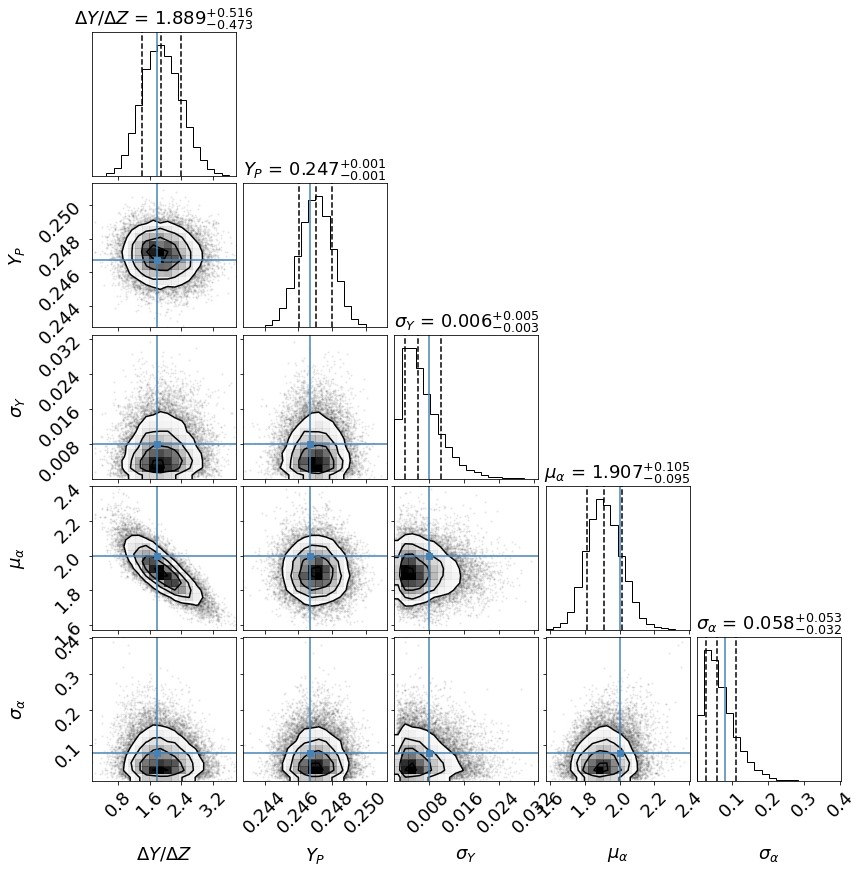
\includegraphics[width=\linewidth]{figures/corner_plot_pp_truths.png}
    \caption[Corner plot showing the marginalised and joint posterior distributions between the PP model hyperparameters for 100 synthetic stars.]{Corner plot showing the marginalised and joint posterior distributions between the PP model hyperparameters for 100 synthetic stars. The true values are shown by the blue lines.}  
    \label{fig:test-corners-pp}   
\end{figure}

In Fig. \ref{fig:test-corners-pp}, we see that the PP model also recovers the hyperparameter truths well, with some noise due to random realisation error. Fitting the model this way has the added benefit over the NP model of improving the inference of the individual stellar parameters, as shown in the previous two sections. We also found that when we ran the PP model with 10 and 50 stars, the uncertainties on the hyperparameters also shrank with increasing $N_\mathrm{stars}$.

\begin{figure}
    \centering
    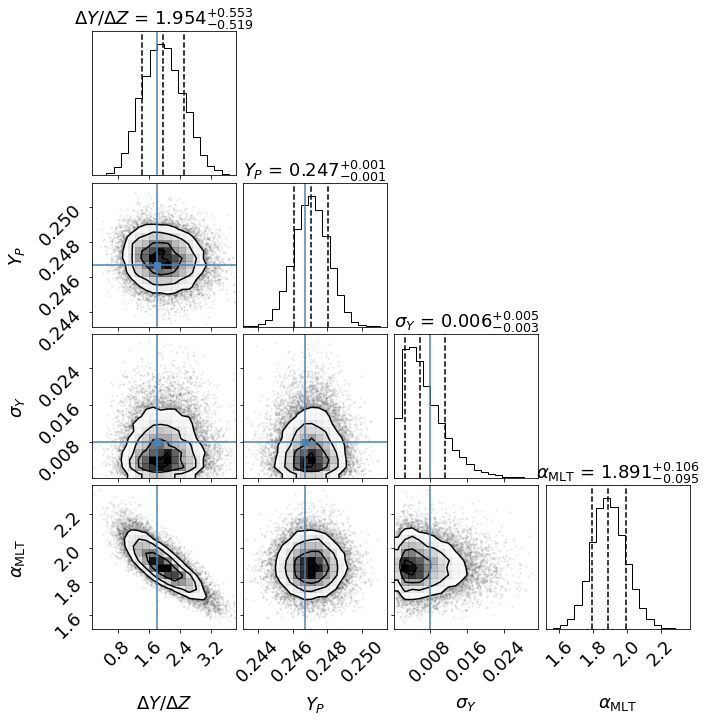
\includegraphics[width=0.82\linewidth]{figures/corner_plot_mp_truths.png}
    \caption{The same as Fig. \ref{fig:test-corners-pp} but for the MP model.}
    \label{fig:test-corners-mp} 
\end{figure}

Fig. \ref{fig:test-corners-mp} shows the hyperparameter results for the MP model. Here, $\mlt$ was assumed to be the same for all stars. This model also recovers the true hyperparameters for helium well, and the assumed value for $\mlt$ is within uncertainty of the true $\mu_\alpha$.

\section{The Sun as a Star}\label{sec:sun-res}

%%%%%%%%%%%%%%%%%%%%%%%%%%%%%%%%%%%%%%%%%%%%%%%%%%

%%%%%%%%%%%%%%% THE SUN AS A STAR %%%%%%%%%%%%%%%%

Our model consistently recovers the Sun when modelled in each of the NP, PP, and MP models. In Table \ref{tab:sun-out} we present the results for the Sun as a star from the NP model to show what we obtain without the influence of any other stars in the sample. We show the marginal and joint posterior distributions for the solar parameters from the NP model in the corner plot in Fig. \ref{fig:sun-results}.

We found some differences between $\mlt$ from our solar model and solar calibrations in the literature produced using \textsc{MESA} with similar input physics. For example, the solar calibration in \citet{Stancliffe.Fossati.ea2016} using \citet{Asplund.Grevesse.ea2009} abundances yields compatible initial abundances, $Z_\mathrm{init} = 0.0149$ and $Y_\mathrm{init} = 0.266$ but $\mlt = 1.783$ which differs from our results by about 10-$\sigma$. This is likely because of a few differences in observed values used for the calibration. \citet{Stancliffe.Fossati.ea2016} used observed helium abundance and convection zone depth measurements from helioseismology. Furthermore, solar calibrations typically include convective envelope overshooting. Presuming overshooting increases mixing in the star, we might expect a lower $\mlt$ to compensate this. Therefore, we stress that the addition of the Sun as a star in our model is with the assumption of our choice of input physics.

\begin{table}
    \centering
    \caption[Solar results from the NP model.]{Solar results from the NP model. The second column shows the median marginalised posterior samples for each parameter with their respective upper and lower 68 per cent credible intervals.}
    \label{tab:sun-out}
    \subcaption*{Input parameters.}
\begin{tabular}{ccccc}
\toprule
                  $f_\mathrm{evol}$ &              $M\,(\si{\solarmass})$ &                           $\mlt$ &                   $Y_\mathrm{init}$ &                      $Z_\mathrm{init}$ \\
\midrule
 $0.517\substack{+0.009 \\ -0.008}$ &  $1.000\substack{+0.001 \\ -0.001}$ &  $2.12\substack{+0.03 \\ -0.03}$ &  $0.262\substack{+0.002 \\ -0.002}$ &  $0.0150\substack{+0.0003 \\ -0.0003}$ \\
\bottomrule
\end{tabular}
\bigskip
\subcaption*{Output parameters.}
\begin{tabular}{ccccc}
    \toprule
                      $\tau\,(\si{\giga\year})$ &      $\teff\,(\si{\kelvin})$ &            $R\,(\si{\solarradius})$ &        $\dnu\,(\si{\micro\hertz})$ & $\metallicity_\mathrm{surf}\,(\si{\dex})$ \\
    \midrule
     $4.6\substack{+0.1 \\ -0.1}$ &  $5777\substack{+12 \\ -12}$ &  $1.001\substack{+0.001 \\ -0.001}$ &  $135.37\substack{+0.14 \\ -0.14}$ &           $0.00\substack{+0.01 \\ -0.01}$ \\
    \bottomrule
    \end{tabular}
\end{table}

\begin{figure}
    \centering
    \includegraphics[width=\textwidth]{figures/corner_plot_sun.png}
    \caption{A corner plot showing the sampled marginal and joint posterior distributions for the Sun as a part of the NP model.}
    \label{fig:sun-results}
\end{figure}

%%%%%%%%%%%%%%%%%%%%%%%%%%%%%%%%%%%%%%%%%%%%%%%%%%
